\chapter{Вступ}
\section{Теоретичні відомості до першого завдання}
\subsection{Алгебра логіки}
\textbf{Алгебра логіки} \emph{(Булева логіка, двійкова логіка, двійкова алгебра)} — розділ математичної логіки, що вивчає систему логічних операцій над висловлюваннями. Вважається, що висловлювання можуть бути тільки істинними або помилковими, тобто використовується так звана \emph{бінарна або двійкова логіка}.

Булева функція задається у вигляді таблиці, або графіка зі стандартним (лексикографічним) розташуванням наборів аргументів,виконана кодом Грея.

\textbf{Код Грея} — одна із систем кодування інформації, в якій два послідовні коди відрізняються значенням лише одного біта.

\textbf{Табли́ця істинності} — математична таблиця, що широко використовується у математичній логіці зокрема в алгебрі логіки, численні висловлень для обчислення значень булевих функцій.

Приклад таблиці істинності:
\newpage
\subsection{Базові логічні вирази}
Відомі такі основні логічні вирази, як:
\begin{itemize}
	\item Інверсія (логічне  'НЕ', NOT,$\lnot$)
	\item Кон'юнкція (логічне множення, логічне  'І', AND,$\wedge$)
	\item Диз'юнкція (логічне додавання, логічне  'АБО', OR,$\lor$)
\end{itemize}

Також існують комбіновані логічні вирази:
\begin{itemize}
	\item І-НЕ(NAND,$\uparrow$)
	\item АБО-НЕ(NOR,$\downarrow$)
	\item Мod2(XOR,$\oplus$)
\end{itemize}
\newpage
\subsection{Форма подання логічних виразів}
Логічний вираз який є тотожний функції можна подати у трьох загальних виглядах:
\begin{itemize}
	\item Диз'юнктивна нормальна форма (ДНФ)
	\item Кон'юнктивна нормальна форма (КНФ)
	\item Алгебраїчна нормальна форма (АНФ або поліном Жегалкіна)
\end{itemize}
\newpage
\subsection{Мінімізація логічних виразів}
Для логічних виразів існують такі закони алгебри:
\begin{center}
\begin{table}[h!]
\begin{tabu} { | X[3,с] | X[3,c] | X[3,c] | }
 \hline
Назва закону& АБО & І \\
 \hline
 Переміщення &  &  \\
\hline
 Комбінування &  &    \\
\hline
Розподільний &  &   \\
\hline
Ідемпотентність & &   \\
\hline
Виключення & &   \\
\hline
Операції з константами & &   \\
\hline
Поглинання & &   \\
\hline
Склеювання& &   \\
\hline
Контрпозиція& &   \\
\hline
Подвійне заперечення& &   \\
\hline
Спрощення& &   \\
\hline 
\end{tabu}
\vspace{6mm}\\
\caption{Таблиця законів алгебри логічних виразів}\label{tab:logic}
\end{table}
\end{center}

Існують інші способи мінімізації логічних виразів такі, як карти Карно і метод Куайна — Мак-Класкі, але вони не будуть розглядаться в данній роботі.
\newpage
\section{Теоретичні відомості до другого завдання}

\newpage
\chapter{Перше завдання}
\section{Перша функція}
\newpage
\subsection{Мінімізація та побудова схеми функції}

\newpage
%\includepdf[pages=-]{scheme_1.1.pdf}
\subsection{Переведення в базис І-НЕ(NAND) та побудова схеми функції}
 
\newpage
%\includepdf[pages=-]{scheme_1.1.1.pdf}
\subsection{Переведення в базис АБО-НЕ(NOR) та побудова схеми функції}
 
\newpage
%\includepdf[pages=-]{scheme_1.1.2.pdf}
\section{Друга функція}

\newpage
\subsection{Мінімізація та побудова схеми функції}

\newpage
%\includepdf[pages=-]{scheme_1.2.pdf}
\subsection{Переведення в базис І-НЕ(NAND) та побудова схеми функції}

\newpage
%\includepdf[pages=-]{scheme_1.2.1.pdf}
\subsection{Переведення в базис АБО-НЕ(NOR) та побудова схеми функції}

\newpage
%\includepdf[pages=-]{scheme_1.2.2.pdf}
\chapter{Друге завдання}
\section{Характеристики дешифратора}

\newpage
\subsection{Таблиця адресних просторів та схема неповного дешифратора}

\newpage
%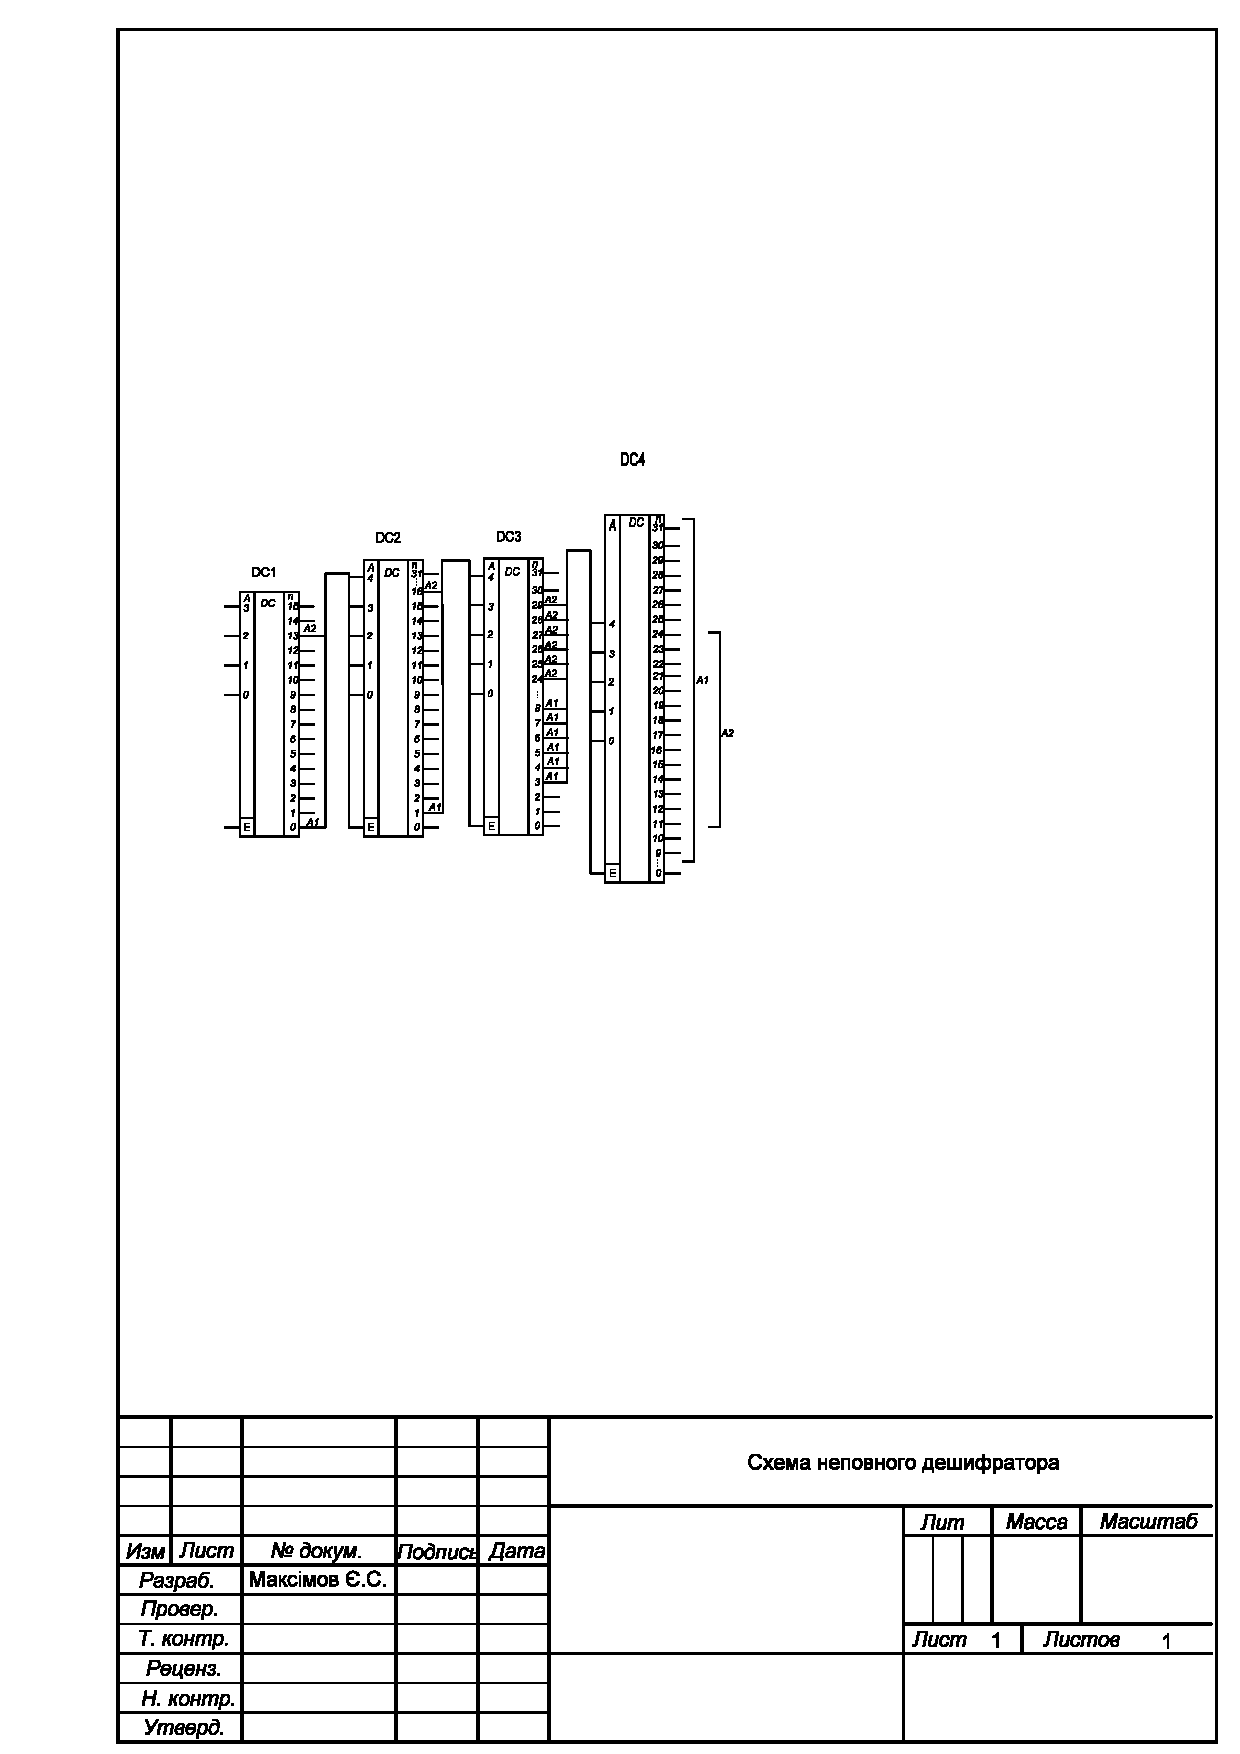
\includepdf[pages=-]{scheme_2.pdf}
\section{Апаратні витрати на побудову дешифратора}

\newpage
\chapter{Висновок}
